\documentclass{report}
\usepackage[pdftex]{graphicx}
\usepackage{sidecap}
\usepackage{fancyhdr}
\usepackage{lscape}
\usepackage[francais]{babel} 
\usepackage[absolute]{textpos}
\usepackage{amssymb}


\usepackage[utf8]{inputenc}  
\usepackage[T1]{fontenc}


\title{Rapport de labo d'\'electronique: \\ Circuits logiques}
\author{Groupe ?: \\ Mattens Simon; Dom Eduardo \\ BA2 Info}
\date{Labo r\'ealis\'e le 3 mai 2018}

\pagestyle{fancy}
\lhead{Groupe ?: Mattens S. ; Dom E.}
\rhead{BA2 Info}
\cfoot{\thepage}
\begin{document}
\maketitle




\section*{1 Introduction}

\hspace*{1,5cm}Le but de ce tp est de comprendre et d'\^etre capable de construire des fonctions logiques et de construire des circuits éléctroniques basés sur ces notions de fonctions logiques.\\

\section*{2 R\'esum\'e Th\'eorique}
\subsection*{2.1 Les fonctions logiques}
\hspace*{1,5cm} Une fonction logique est une fonction d'une ou de plusieurs variables binaires de valeurs égales à 0 ou 1. Elles sont données pour toute les combinaisons possibles des valeurs des variables binaires dont elle dépend par une table de vérité.\\
Une variable binaire est une variable ne pouvant prendre que 2 valeurs (0 ou 1)\\. 


\subsection*{2.2 Les fonctions logiques \'elementaires}
On retrouve 4 op\'erations logiques \'elementaires:
\begin{enumerate}
\item L'op\'eration NOT(non) qui est \'equivalent \`a la fonction $ \in\overline{A}$ . Elle vaut donc 0 quand x$\in$A et 1 quand x$\in\overline{A}$.\\
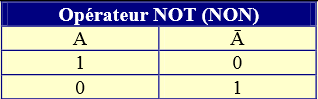
\includegraphics[scale=1]{not.png} 

\newpage

\item L'op\'eration AND(et) correspond au produit logique A.B. Elle vaut 1 quand A$\cup$B est vrai , 0 sinon.\\
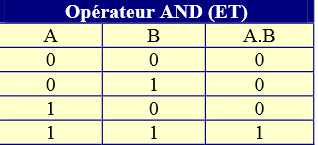
\includegraphics[scale=1]{and.png} 
\item L'op\'eration OR(ou) correspond \`a la somme logique A+B. Elle vaut 1 quand A$\cap$B est vrai, 0 sinon.\\
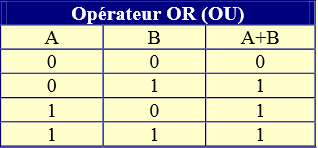
\includegraphics[scale=1]{or.png} 
\item L'operation XOR(ou exclusif) correspond \`a la somme directe A$\oplus$B. Elle vaut 1 quand (A$\cap\overline{B}$)$\cup$($\overline{A}\cap$B).\\
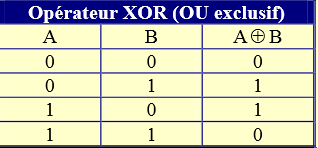
\includegraphics[scale=1]{xor.png} 
\end{enumerate}
On retrouve aussi des fonctions logiques telles que NAND (NON-ET) et NOR (NON-OU).
\newpage
\subsection*{2.3 Les circuits logiques}

Un circuit logique est un circuit électrique ou électronique matérialisant une fonction logique. Ainsi les 2 positions d'un interrupteur à 2 directions peuvent représenter les 2 valeurs d'une variable binaire (0 ou 1), il en est de même pour les 2 états de fonctionnement d'une diode.\\
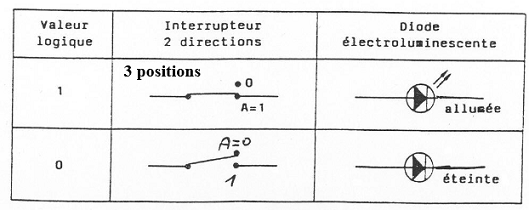
\includegraphics{CirLo.png} \\



\section*{3 Dispositif exp\'erimental}
Le boitier dispose des \'elements suivants:
\begin{itemize}
\item 4 interrupteurs à 2 directions et munis de LEDs indiquant l'état "haut" ou "bas", à définir en tant que "o" ou "1".
\item 4 LEDs de contr\^ole de couleur différente et indépendantes dont la fonction est de déterminer l'état du circuit établi.
\item une plaquette de connexion.
\item Des boutons poussoirs
\end{itemize}

Le circuit int\'egr\'e SN7400 comporte 4 circuits logiques simples identiques (représentés par un même pictogramme). Nous devrons déterminer le type de fonction logique réalisée par chacun de ces circuits de base lors du tp.\\
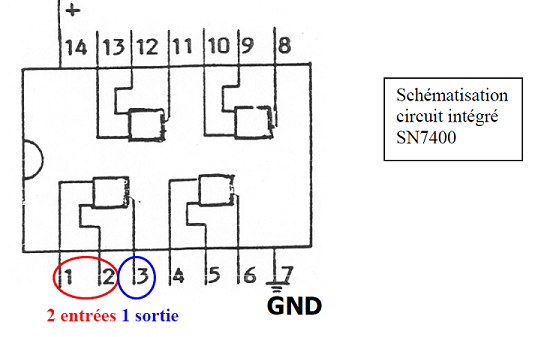
\includegraphics[scale=1]{CirInt.png} 

\newpage

\subsection*{3.2 Les circuits}
Nous avons réalisé les circuits suivants dans la premi\`ere exp\'erience :\\
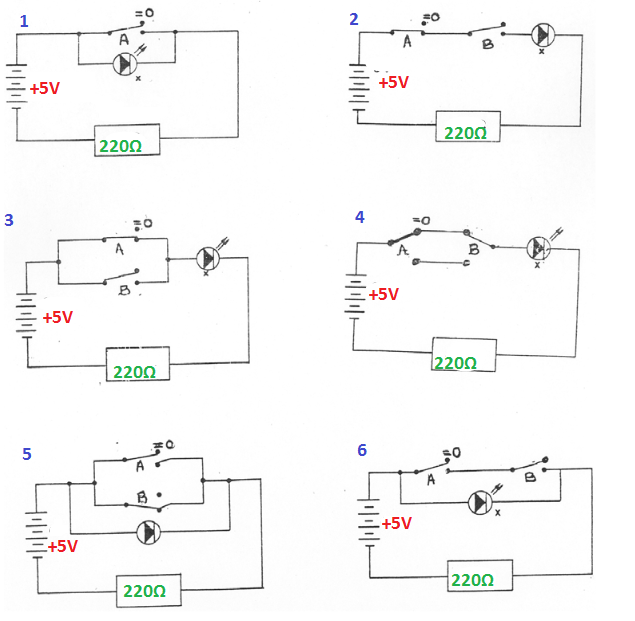
\includegraphics[scale=0.7]{Circuits_1.png} 
\\
\newpage
Pour la seconde exp\'erience nous avons fait les circuits suivants: \\
\subsubsection*{3.2.1 Premier circuit}
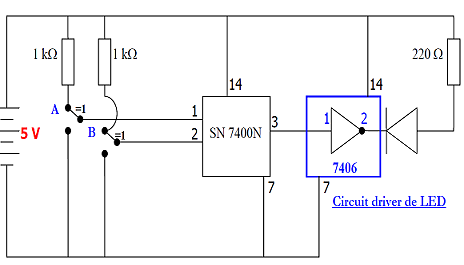
\includegraphics[scale=1]{CirInt1.png} 
\subsubsection*{3.2.2 Court-circuitage}
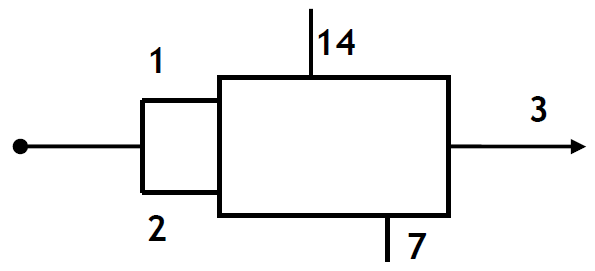
\includegraphics[scale=1]{Court-circuit.png} 
\subsubsection*{3.2.3 Les Montages}
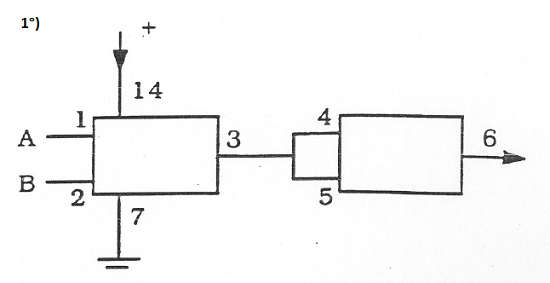
\includegraphics[scale=1]{CirInt2.png} 
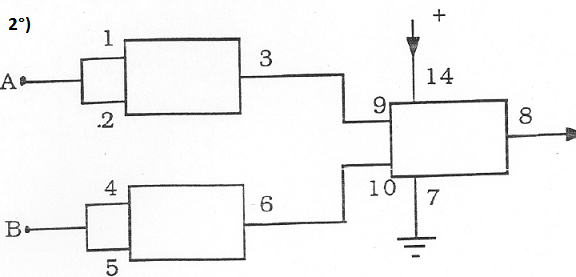
\includegraphics[scale=1]{CirInt3.png} 
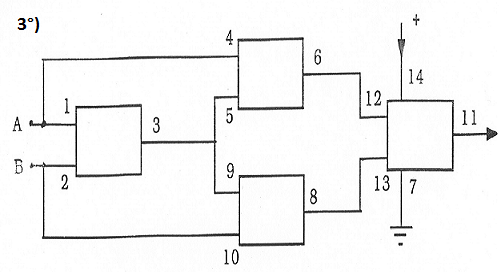
\includegraphics[scale=1]{CirInt4.png} 
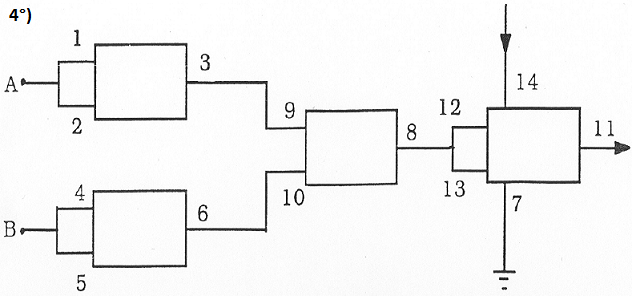
\includegraphics[scale=1]{CirInt5.png} 
\newpage

\section*{4 Prise des mesures et résultats}
\subsection*{4.1 Premi\`ere exp\'erience}
\subsubsection*{4.1.1 Pr\'evision des r\'esultats}
\begin{enumerate}
\item Vu que l'interrupteur est en parall\`ele avec la LED, on peut pr\'edire que si celui-ci est ferm\'e alors le courant passera par cet interrupteur et pas par la LED (la résistance à l'intérieur de la LED est plus grande que celle de l'interrupteur). Nous pensons que la fonction logique est donc un NON.
\item les 2 interrupteurs et la LED sont en série, les deux interrupteurs doivent \^etre ferm\'es pour que le courant passe. Nous pensons que la fonction logique est donc un ET.
\item Pour que le courant passe dans la LED, le courant doit passer soit dans l'interrupteur A, soit dans le B ou dans les deux. Nous pensons que la fonction logique est donc un OU.
\item Pour que le circuit soit ferm\'e, il faut les deux interrupteurs soient dans la m\^eme position. Nous pensons que la fonction logique est donc un NON-XOR.
\item Vu que les interrupteurs sont en parall\`eles par rapport \`a la LED parall\`eles et eux mêmes parallèles entre eux, la LED ne s'allumera que si les deux interrupteurs sont ouverts. Nous pensons que la fonction logique est donc un NON-OU.
\item Vu que les deux interrupteurs sont en parallèles avec la LED et qu'ils sont en s\'erie entre eux, la LED ne s'allumera que si l'un des deux interrupteurs est ouvert. Nous pensons que la fonction logique est donc un NON-ET.
\end{enumerate}
\subsection*{4.1.2 Exp\'erimentation}
\begin{enumerate}
\item La LED est allum\'ee lorsque le bouton A est ouvert, \'eteinte si le bouton A est ferm\'e.
\item La LED est allum\'ee si les deux boutons sont ferm\'es , \'eteinte sinon.
\item La LED est \'eteinte si les deux boutons sont ouverts, allum\'ee sinon.
\item La LED est allum\'ee si les deux boutons sont sur la m\^eme position, \'eteinte sinon.
\item La LED n'est allum\'ee que si les deux boutons sont ouverts, \'eteinte sinon.
\item La LED n'est \'eteinte que si les deux boutons sont ferm\'es, allum\'ee sinon.

\end{enumerate}

\textbf{\'Enonc\'e:} La convention relative aux interrupteurs est-elle importante ?. \\


\textbf{R\'eponse:}  \\
Oui sinon il faudrait changer les portes logiques.

\newpage
\subsection*{4.2 Seconde Expérience : Etude de circuist int\'egr\'es logiques}
\subsubsection*{4.2.1 Premier circuit}
\hspace*{1,5cm} La LED n'est \'eteinte que si les deux boutons sont ferm\'es, allum\'ee sinon. La fonction logique correspondant au circuit est un NON-ET.Ce qui donne la table suivante:\\
\begin{tabular}{|c|c|c|}
\hline
A & B & S \\
\hline
1&1&0\\
1&0&1\\
0&1&1\\
0&0&1\\
\hline
\end{tabular}\\
\subsubsection*{4.2.2 Court-circuitage les entr\'ees}
\hspace*{1,5cm} Si on court-circuite les entr\'ees 1 et 2,on obtient la table
suivante:\\
\begin{tabular}{|c|c|}
\hline
A & S \\
\hline
1&0\\
0&1\\
\hline
\end{tabular}\\
\subsubsection*{4.2.3 Les montages}
\begin{enumerate}
\item La LED est allum\'ee si les deux boutons sont ferm\'es , \'eteinte sinon. L'opérateur logique représenté est le ET.
\item La LED est \'eteinte si les deux boutons sont ouverts, allum\'ee sinon. L'opérateur logique représenté est le OU.
\item La LED est allum\'ee si les deux boutons sont dans des \'etats inverses(l'un ouvert, l'autre ferm\'e), \'eteinte sinon. L'opérateur logique représenté est le XOR.
\item La LED est allum\'ee si les deux boutons sont ouverts, \'eteinte sinon. L'opérateur logique représenté est le NOR.
\end{enumerate}
\newpage

\section*{5 Analyse des r\'esultats}
\subsection*{5.1 Préambule}
\subsubsection*{5.1.1 Démontrer que A$\oplus$B = A.$\overline{B}$ + $\overline{A}$.B}
\hspace*{1,5cm} Afin de prouver que A$\oplus$B = A.$\overline{B}$ + $\overline{A}$.B est une tautologie, construisons la table de v\'erit\'e de l'expression.\\
\begin{tabular}{|c|c|c|c|c|c|c|c|}
\hline
 & & & & & & & \\ 
A & B & $\overline{A}$ & $\overline{B}$ & A.$\overline{B}$ & $\overline{A}$.B & A.$\overline{B}$ + $\overline{A}$.B & A$\oplus$B \\
\hline
0&0&1&1&0&0&0&0\\
0&1&1&0&0&1&1&1\\
1&0&0&1&1&0&1&1\\
1&1&0&0&0&0&0&0\\
\hline
\end{tabular}\\
\\
\hspace*{1,5cm} Nous voyons via cette table de v\'erit\'e que A.$\overline{B}$ + $\overline{A}$.B = A$\oplus$B.\\
\subsubsection*{5.1.2 Table NAND et démontrer que $\overline{A.B}$=$\overline{A}+\overline{B}$}
Table NAND: \\
\begin{tabular}{|c|c|c|c|}
\hline
  & & & \\
 A & B & A.B & $\overline{A.B}$\\
\hline
 0 & 0 & 0 & 1\\
 0 & 1 & 0 & 1\\
 1 & 0 & 0 & 1\\
 1 & 1 & 1 & 0 \\
 \hline
\end{tabular} \\

\hspace*{1,5cm}Afin de prouver que $\overline{A.B}$=$\overline{A}+\overline{B}$ est une tautologie ,construisons la table de v\'erit\'e de l'expression.\\

\begin{tabular}{|c|c|c|c|c|c|c|}
\hline
 & & & & & & \\
 A & B & $\overline{A}$ & $\overline{B}$ & $\overline{A}+\overline{B}$ & A.B & $\overline{A.B}$\\
 \hline
 0&0&1&1&1&0&1\\
 0&1&1&0&1&0&1\\
 1&0&0&1&1&0&1\\
 1&1&0&0&0&1&0\\
 \hline
\end{tabular}\\
\hspace*{1,5cm} Nous avons prouv\'e via cette table que l'expression $\overline{A.B}$=$\overline{A}+\overline{B}$ est une tautologie.\\
\newpage
\subsubsection*{5.1.3 Table NOR et démontrer que $\overline{A+B}$=$\overline{A}.\overline{B}$}

\hspace{1,5cm}Table NOR: \\

\begin{tabular}{|c|c|c|c|}
\hline
 & & & \\
 A & B & A+B & $\overline{A+B}$\\
 \hline
 0 & 0 & 0 & 1\\
 0 & 1 & 1 & 0\\
 1 & 0 & 1 & 0\\
 1 & 1 & 1 & 0 \\
 \hline
\end{tabular}\\

\hspace*{1,5cm}Afin de prouver que $\overline{A+B}$=$\overline{A}.\overline{B}$ est une tautologie ,construisons la table de v\'erit\'e de l'expression.\\

\begin{tabular}{|c|c|c|c|c|c|c|}
\hline
 & & & & & & \\ 
A & B & $\overline{A}$ & $\overline{B}$ & $\overline{A}$.$\overline{B}$ & A+B & $\overline{A+B}$ \\
\hline
0&0&1&1&1&0&1\\
0&1&1&0&0&1&0\\
1&0&0&1&0&1&0\\
1&1&0&0&0&1&0\\
\hline
\end{tabular}\\

\hspace*{1,5cm} Nous avons prouv\'e via cette table que l'expression $\overline{A+B}$=$\overline{A}.\overline{B}$ est une tautologie.\\
\newpage

\subsection*{5.2 Premi\`ere exp\'erience}
\begin{enumerate}
\item On obtient les r\'esultats suivant:\\
\\
\begin{tabular}{|c|c|}
\hline
A & LED \\
\hline
0&1\\
1&0\\
\hline
\end{tabular}\\
\hspace*{1,2cm} Ce qui correspond \`a l'opérateur NON.
\item On obtient les résultats suivants:\\
\\
\begin{tabular}{|c|c|c|}
\hline
A & B & LED \\
\hline
0&0&0\\
0&1&0\\
1&0&0\\
1&1&1\\
\hline
\end{tabular}\\
\\
\hspace*{1,2cm} Ce qui correspond \`a l'opérateur ET.
\item On obtient les résultats suivants:\\
\\
\begin{tabular}{|c|c|c|}
\hline
A & B & LED \\
\hline
0&0&0\\
0&1&1\\
1&0&1\\
1&1&1\\
\hline
\end{tabular}\\
\\
\hspace*{1,2cm} Ce qui correspond \`a l'opérateur OU.
\item On obtient les résultats suivants:\\
\\
\begin{tabular}{|c|c|c|}
\hline
A & B & LED \\
\hline
0&0&1\\
0&1&0\\
1&0&0\\
1&1&1\\
\hline
\end{tabular}\\
\hspace*{1,2cm} Ce qui correspond \`a l'opérateur NON XOR.
\item On obtient les résultats suivants:\\
\\
\begin{tabular}{|c|c|c|}
\hline
A & B & LED \\
\hline
0&0&1\\
0&1&0\\
1&0&0\\
1&1&0\\
\hline
\end{tabular}\\
\\
\hspace*{1,2cm} Ce qui correspond \`a l'opérateur NON-OU.
\newpage
\item On obtient les résultats suivants:\\
\\
\begin{tabular}{|c|c|c|}
\hline
A & B & LED \\
\hline
0&0&1\\
0&1&1\\
1&0&1\\
1&1&0\\
\hline
\end{tabular}\\
\\
\hspace*{1,2cm} Ce qui correspond \`a l'opérateur NON-ET.
\end{enumerate}

\subsection*{5.2 Seconde expérience : circuits int\'egr\'es logiques}
\subsubsection*{5.2.1 Premier circuit}
\hspace*{1,5cm} Les \'etats correspondent au tableau de v\'erit\'e du sixi\`eme circuit de la premi\'ere exp\'erience. Nous avons donc une fonction logique NON-ET:
\begin{tabular}{|c|c|c|}
\hline
A & B & S \\
\hline
1&1&0\\
1&0&1\\
0&1&1\\
0&0&1\\
\hline
\end{tabular}\\
\\
\subsubsection*{5.2.2 Court-circuitage des entr\'ees 1 et 2}
\hspace*{1,5cm} Lors du court-circuitage , obtient une fonction logique NON. En effet, nous avons:\\
\\
\begin{tabular}{|c|c|}
\hline
A&S  \\
\hline
0&1\\
1&0\\
\hline
\end{tabular}\\
\\
\hspace*{1,5cm} Ce qui correspond \`a un NON.
\subsubsection*{5.2.3 Les Montages}
\begin{enumerate}
\item Lors du premier montage on obtient:\\
\\
\begin{tabular}{|c|c|c|}
\hline
A & B & LED \\
\hline
0&0&0\\
0&1&0\\
1&0&0\\
1&1&1\\
\hline
\end{tabular}\\
\\
Ce qui correspond \`a la fonction logique ET.\\
\newpage
\item Lors du Deuxi\`eme montage, on obtient:\\
\begin{tabular}{|c|c|c|}
\hline
A & B & LED \\
\hline
0&0&0\\
0&1&1\\
1&0&1\\
1&1&1\\
\hline
\end{tabular}\\
Ce qui correspond \`a la fonction logique OU.\\
\item Lors du Troisi\`eme montage on obtient:\\
\\
\begin{tabular}{|c|c|c|}
\hline
A & B & LED \\
\hline
0&0&0\\
0&1&1\\
1&0&1\\
1&1&0\\
\hline
\end{tabular}\\
\\
Ce qui correspond \`a la fonction logique XOR.
\item Lors du Quatrième montage, on obtient :\\
\\
\begin{tabular}{|c|c|c|}
\hline
A & B & LED \\
\hline
0&0&1\\
0&1&0\\
1&0&0\\
1&1&1\\
\hline
\end{tabular}\\
\\
Ce qui correspond \`a la fonction logique NOR.
\end{enumerate}


\section*{6 Conclusion}
\hspace*{1,5cm} Nous avons  construit de nombreux circuits correspondant aux portes logiques \'el\'ementaire. Nous avons donc prouv\'e que chaque fonction logique pouvait \^etre construit sous la forme d'un circuit logique gr\^ace \`a des interrupteurs et des LEDs vérifiant ces portes logiques.\\


\end{document}